

Collections are fundamental to most programming tasks because they allow the user to group and process large sets of data.
However, when it comes to expressing moderately complex collection manipulations, C++ is markedly behind some of its more modern counterparts with respect to code clarity and efficiency of space.
This is the problem we set out to solve.

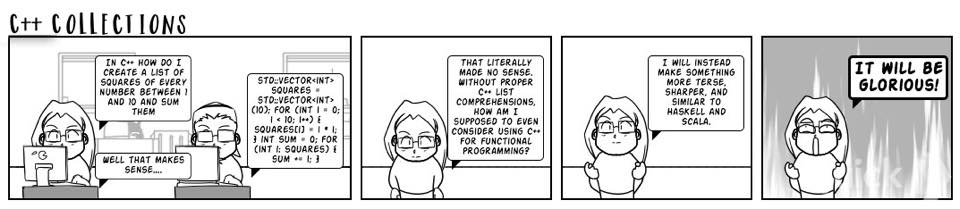
\includegraphics[width=\textwidth]{comic}


Languages are used as tools to communicate, and consequently, the structure and limitations of the languages we use determine the way we think.
This idea, known in the field of linguistic relativity as the Sapir-Whorf hypothesis\cite{linguistic_relativity}, has critical implications when applied to programming languages, namely that the ability of a programmer to reason about a problem can be limited by the languages he or she has learned (or has yet to learn).
Furthermore, if we hold this hypothesis to be true, we can reasonably conclude that learning how to write code in a new language can provide a programmer with a totally new way of thinking about solving a problem that he or she may have already solved a dozen times before.

C++ is an interesting language in this respect because in recent years it has begun to introduce new language constructs that help it blur the lines between programming paradigms along which programming languages are usually divided.
Perhaps most notably, C++11 introduced a set of features that allows for functional programming in the language.
Functional programming is a programming paradigm that avoids state and favors immutable variables.
It is as if the English language introduced a new group of words, whose meanings were all missing from the original dictionary.
The conclusion we are tempted to draw from this addition is that C++ is a great language to learn, because its new functional vocabulary will allow the programmer who learns it to think about problems both from a traditional C++ perspective, and now also from a functional perspective.

Unfortunately, the ease of use of many of C++'s functional features pales in comparison to that of other functional languages, making it daunting for beginners in functional programming to use the features correctly, if at all.

\blockquote{In 24 hours you might be able to learn some of the syntax of C++ (if you already know another language), but you couldn't learn much about how to use the language. In short, if you were, say, a Basic programmer, you could learn to write programs in the style of Basic using C++ syntax, but you couldn't learn what C++ is actually good (and bad) for. So what's the point? Alan Perlis once said: "A language that doesn't affect the way you think about programming, is not worth knowing" -- Peter Norvig\cite{norvig}
}

C++ Collections is a library built on top of C++11 that provides both finite and infinite collections data structures, built from the ground up with syntax in mind.
It strives to make functional programming concepts, specifically to do with lists, more accessible and understandable to C++ programmers.

An additional perk of functional languages is the terseness associated with them.
Software bugs per line of code have been found to be constant across different languages\cite{code_complete} which indicates that more succint operations on lists are more likely to operate as intended.

To use the C++ Collections library, download it from Github and simply \code{\#include cpp\_collections.h} in your source file.

